\section{Blender}
\label{sec:chapter_tecnologie_abilitanti_blender}

Blender è un software di computer grafica 3D professionale, gratuito ed open source. 
Viene utilizzato maggiormente per la creazione di film animati, effetti visivi, applicazioni 3D interattive e videogiochi \cite{blender} . 
Supporta interamente la pipeline 3D ed offre varie funzionalità avanzate come la modellazione 3D, la mappatura UV, l’ unwrap, la texturizzazione di oggetti, la simulazione di particelle, animazioni, rendering.
Il software dispone di un interprete interno Python grazie al quale offre delle API per la creazione ed esecuzione di script Python. 
Tali script permettono la realizzazione di applicazioni personalizzate in base ai propri interessi.
Python è un linguaggio di programmazione interpretato, interattivo ed orientato agli oggetti che comprende moduli, eccezioni, gestione dinamica dei tipi e classi. Inoltre le variabili non sono tipizzate e l’indentazione è necessaria per definire i blocchi.
Questa funzionalità di scripting è stata essenziale in questo lavoro di tesi per la creazione, tra le altre cose, di un tool che effettuasse il processo di baking in maniera automatica. Il tool verrà esaminato nei capitoli successivi.
Il software Blender è multi-piattaforma e compatibile con i sistemi operativi Linux, Windows e Macintosh.
\\
Attualmente il motore di default per il render è il Blender Render. Esso è un motore di tipo Biased in cui il calcolo della luce avviene secondo un’approssimazione visiva; viene calcolata la dimensione degli oggetti e la distanza delle luci, e da queste si ricavano ombre ed illuminazione.
Il punto di forza di questo tipo di motore è il totale controllo sulla luce ma può richiedere molta esperienza in campo fotografico ed artistico per poter essere padroneggiato. Ulteriore caratteristica positiva è l’efficienza; il motore permette di ottenere anteprime di rendering in minore tempo rispetto ad algoritmi di tipo Unbiased, come il path tracing.
Questo tipo di soluzione è però fisicamente non corretta in quanto non calcola i rimbalzi di luce sugli oggetti, non permettendo quindi di ottenere ombre e luci realistiche.
\\
Blender ha un ulteriore motore di render di tipo Unbiased chiamato Cycles, il quale permette di ottenere un’illuminazione fisicamente più corretta dei motori Biased.
Nel presente lavoro di tesi è stato scelto questo motore di rendering in quanto, a differenza del Blender Render, permette di ottenere sugli oggetti presenti nella scena degli effetti di luci ed ombre estremamente realistici; paragonabili a quelli nel mondo reale.
\begin{figure}[htb]
 \centering
 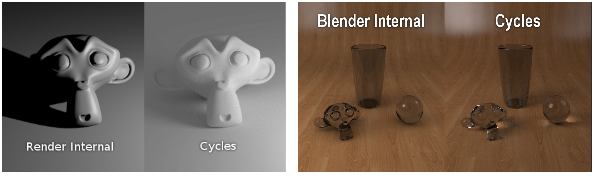
\includegraphics[width=0.9\linewidth]{images/chapter_tecnologie_abilitanti/tecnologie_abilitanti_bias_unbias.png}\hfill
 \caption[Cycles render e Blender render]{Confronto tra ombre e luci ottenute mediante Blender render (Unbiased) e Cycles render (Biased)}
 \label{fig:tecnologie_abilitanti_bias_unbias}
\end{figure}
Per modificare i materiali degli oggetti, le texture, ed il rendering in generale, Blender permette una metodologia di programmazione molto potente e flessibile, grazie al Node Editor. Tale strumento ha permesso di lavorare con il Cycles Renderer con estrema facilità ed è stato essenziale per permettere la creazioni di materiali complessi. \cite{node_editor1,node_editor3}
\\
\begin{figure}[htb]
 \centering
 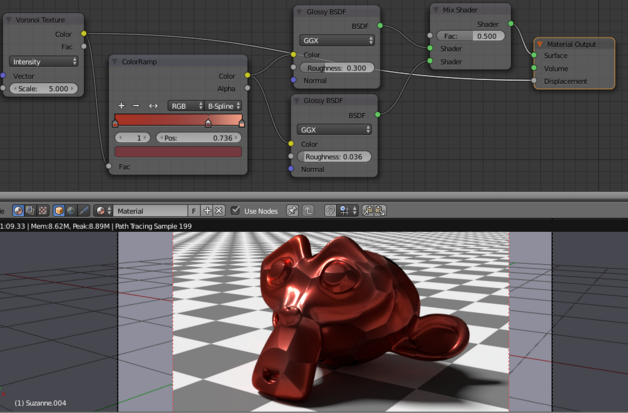
\includegraphics[width=1\linewidth]{images/chapter_tecnologie_abilitanti/tecnologie_abilitanti_node_editor.png}\hfill
 \caption[Blender Node Editor]{Il Node Editor di Blender}
 \label{fig:tecnologie_abilitanti_node_editor}
\end{figure}
Cycles correntemente supporta un integratore path tracing che funziona bene per la maggior parte degli effetti luce, ma non è cosi adatto per effetti caustici ed alcune complesse situazioni di luce. I raggi vengono lanciati dalla camera verso la scena, rimbalzando sulle superfici incontrate fino a quando viene raggiunta una fonte di luce come una lampada, un oggetto che emette luce, o lo sfondo della scena. 
Le luci vengono individuate sia tramite sample indiretto, in cui i raggi seguono il proprio percorso ottico fino a quando incontrano una fonte di luce, sia tramite sample di luce diretto, in cui si prende una luce e viene direzionato il raggio verso di essa.
\\
Per sample, come spiegato in precedenza, si intende il numero di raggi di luce che vengono tracciati per ogni pixel e Blender permette di indicare il numero di sample da utilizzare per effettuare il rendering della scena. Maggiore è il sample, migliore e meno rumoroso è il risultato ottenuto con il render.
\\
Nel dettaglio Blender utilizza due diversi integratori: l’integratore path tracer e l’integratore path tracer ramificato (\emph{branched path tracer}).
\\
L’integratore path tracer prevede un approccio classico, esaminato in dettaglio nel capitolo \ref{sec:chapter_stato_arte_ray_tracing}, in cui il raggio di luce ogni volta che colpisce un oggetto nella scena rimbalza in una direzione parzialmente casuale fino a quando non colpisce la fonte luminosa da cui riceve la luce.
Questo rende il singolo sample molto veloce da calcolare, ma ne richiede un numero elevato per ottenere un risultato di rendering pulito e senza rumore.
\begin{figure}[htb]
 \centering
 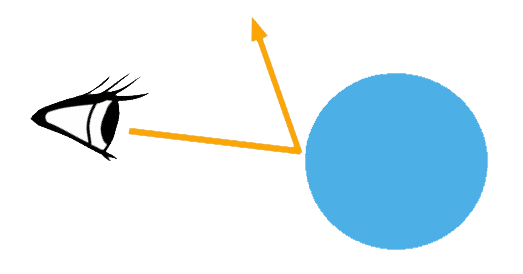
\includegraphics[width=0.6\linewidth]{images/chapter_tecnologie_abilitanti/tecnologie_abilitanti_sferaluce1.jpg}\hfill
 \caption[Integratore path tracer classico]{Integratore path tracer classico in cui il raggio di luce rimbalza in una sola direzione}
 \label{fig:tecnologie_abilitanti_sferaluce1}
\end{figure}
L’integratore path tracer ramificato (formalmente chiamato integratore non progressivo) prevede un approccio differente, in cui il raggio quando colpisce un oggetto  viene diviso in più raggi con direzioni randomiche. Sia la direzione che il numero di raggi in cui viene diviso sono dipendenti dal tipo di materiale di cui è costituito l’oggetto intersecato.
\\
Blender permette nel dettaglio di effettuare, tramite questo integratore, una più precisa parametrizzazione del sample voluto, permettendo di :
\begin{itemize}
\item Specificare il numero di sample da utilizzare, cioè il numero di raggi da lanciare, per ogni pixel del piano immagine tramite l’ attributo AA Render Samples.
\item Specificare un numero differente di sample o di raggi in cui il raggio viene diviso in base al tipo di materiale colpito, tramite gli attributi: \emph{Diffuse Samples}, \emph{Glossy Samples}, \emph{Transmission Samples}. Quindi se ad esempio il Diffuse Samples ha valore 5 mentre il Glossy Samples ha valore 2, il raggio viene diviso 5 volte quando colpisce un oggetto diffuse, mentre viene diviso 2 volte quando ne incontra uno glossy.
\end{itemize}
Questo permette di avere un maggiore controllo sul numero di raggi presenti nella scena e permette di creare configurazioni specifiche in base alla scena da renderizzare.
Se ad esempio in una scena fossero presenti molti oggetti con materiale glossy, ma pochi con materiale di tipo diffuse, il valore dell’attributo glossy samples può essere incrementato rispetto a quello diffuse, in modo da velocizzare il rendering degli oggetti diffuse che incidono poco sul risultato finale.
\\
Ogni sample quindi risulta più lento da calcolare rispetto l’approccio classico ma è richiesto un numero nettamente inferiore di sample per ottenere un risultato di rendering senza rumore.
Ad esempio in una scena in cui sono presenti solo oggetti con materiale diffuse, per ottenere un numero di sample equivalente all’ integratore path tracing classico, che ne utilizza 250, è necessario utilizzare 10 AA samples e 24 Diffuse Samples. Dove 10 x 25 = 250.
\begin{figure}[htb]
 \centering
 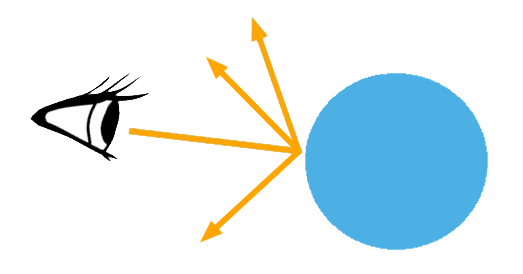
\includegraphics[width=0.6\linewidth]{images/chapter_tecnologie_abilitanti/tecnologie_abilitanti_sferaluce2.jpg}\hfill
 \caption[Integratore path tracer ramificato]{Integratore path tracer ramificato in cui il raggio di luce rimbalza in più direzione}
 \label{fig:tecnologie_abilitanti_sferaluce2}
\end{figure}
Per il presente lavoro di tesi è stato preferito utilizzare l’approccio di path tracing classico per facilitare all’ utilizzatore dell’ applicazione creata l’avvio di questo algoritmo. Egli infatti indicherà solamente un valore di sample senza dover necessariamente conoscere il funzionamento dell’ algoritmo. Algoritmo che avrebbe dovuto comprendere nel caso in cui avesse utilizzato l’approccio ramificato.
Oltre al samples esistono ulteriori parametri per effettuare il rendering ma questi verrano analizzati nel dettaglio nei capitoli successivi.
\\
Infine Blender offre il rendering GPU permettendo di utilizzare la scheda grafica, al posto della CPU, per migliorare notevolmente i tempi di rendering grazie alla maggiore potenza di calcolo.
In particolare Cycles prevede due modalità di rendering GPU:
\begin{itemize}
\item CUDA: l'architettura di elaborazione in parallelo che permette il rendering veloce su schede grafiche NVidia.
\item OpenCL: supporta il rendering su schede grafiche AMD/ATI, però ancora in fase sperimentale.
\end{itemize}
In questo lavoro di tesi è stato utilizzato CUDA per ottenere miglioramenti netti nei tempi di rendering permettendo di velocizzare notevolmente il servizio creato.